\documentclass[a4paper,10pt]{report}

% Packages
\usepackage[utf8]{inputenc}
\usepackage{amsmath, amssymb}
\usepackage{graphicx}
\usepackage{caption}
\usepackage{subcaption}
\usepackage{geometry}
\usepackage{hyperref}
\usepackage{natbib}
\geometry{margin=2.5cm}


\begin{document}

\begin{center}
	{\LARGE\bfseries Bayesian Parameter Estimation of the Network SIS Model using MCMC Methods \par}
	\vspace{0.6cm}
	Banaan Kiamanesh, Pietro Ferraresi, Riccardo Bresolin, Matteo Polo,\\ Mauricio Dada Fonseca De Freitas \\
	May 2025
\end{center}

\vspace{0cm}

\begin{center}
	\textbf{Abstract}
\end{center}
This project implements Bayesian parameter estimation for the Network SIS model using Markov Chain Monte Carlo (MCMC) methods. We aim to estimate key parameters such as network interaction and recovery rates, highlighting the advantages of Bayesian approaches over traditional estimation techniques.


\section{Introduction}

The spread of infectious diseases remains a critical challenge for public health systems worldwide. The SIS model captures the dynamics of diseases where immunity is temporary or non-existent. This makes the SIS framework particularly relevant for ongoing surveillance and control of endemic infections.

Our motivation to focus on the SIS model stems from its wide applicability in modeling the persistence of infectious diseases within a population, especially in interconnected environments such as social networks, transportation systems, or healthcare settings. In these contexts, network-based extensions of the SIS model allow researchers to capture the heterogeneity of contacts and transmission pathways between individuals or subpopulations. Accurate estimation of the SIS model parameters, such as transmission rates and recovery rates, is essential for developing effective intervention strategies, including vaccination, quarantine policies, or resource allocation in healthcare systems.

Lately, the relevance of this topic has been further amplified by "JOINT COMMUNICATION TO THE EUROPEAN PARLIAMENT, THE 
EUROPEAN COUNCIL, THE COUNCIL, THE EUROPEAN ECONOMIC AND 
SOCIAL COMMITTEE AND THE COMMITTEE OF THE REGIONS" a Preparedness Union Strategy to strengthen its ability to handle future pandemics and health crises. Our study aligns with these priorities by focusing on the development of Bayesian parameter estimation methods for the Network SIS model, which can enhance the reliability of epidemiological predictions under uncertainty.

In this project, we aim to implement and test a Bayesian framework for parameter estimation in the Network SIS model using Markov Chain Monte Carlo (MCMC) methods. By leveraging synthetic data and exploring the challenges of numerical identifiability, we aim to demonstrate the advantages of Bayesian approaches over classical estimation techniques and contribute to the broader effort of building resilient, data-informed public health systems.


\section{The Network SIS Model}
\subsection{Model Equations}
Present the SIS model for a network:

\[
\boxed{
\frac{dI}{dt} = \beta I (1 - I) - \gamma I
}
\]
where:
\begin{itemize}
    \item $I(t)$ is the fraction of infected individuals in the population at time $t$,
    \item $\beta$ is the transmission (infection) rate,
    \item $\gamma$ is the recovery rate.
\end{itemize}

The term $\beta I (1 - I)$ represents the rate at which susceptibles become infected, while $\gamma I$ accounts for recovery of infected individuals.



In matrix form, the system can be written compactly as:
\[
\boxed{
\frac{d\mathbf{x}}{dt} = \beta (I_n-\operatorname{diag}(\mathbf{x})) \, A \, \mathbf{x} - \gamma \mathbf{x}
}
\]
where: 
\begin{itemize}
    \item $\mathbf{x} = [x_1, x_2, \dots, x_n]^T$ is the vector of infection fractions across all nodes.
    \item $A = [A_{ij}]$ is the contact rate from node $j$ to node $i$ (the adjacency matrix of the network),
    \item $\gamma$ is the recovery rate, assumed uniform across all nodes.
\end{itemize}


\subsection{Challenges in Parameter Estimation}
Discuss nonlinearity, stochasticity, and potential identifiability issues.

\section{Bayesian Framework for Parameter Estimation}
\subsection{Bayesian Formulation}
Define priors, likelihood, and posterior distribution:
The Bayesian Framework is characterized by three fundamental probability distributions:
\begin{itemize}
    \item \textbf{Prior} ($P(\theta)$): Represents our initial knowledge about the parameters ($\theta$) \emph{before} observing any experimental data;
    \item \textbf{Likelihood} ($P(\text{Data}|\theta)$): Describes the probability of observing the data given specific values of the parameters ($\theta$). It is a function of the parameters that quantifies how well these parameters explain the data.
    \item \textbf{Posterior} ($P(\theta|\text{Data})$): Is the updated probability distribution of the parameters ($\theta$) after observing the data, obtained by combining the prior with the data observed through the likelihood, according to Bayes' Theorem.
\end{itemize}
The specification of prior distributions for the parameters, while not entirely arbitrary, involves an element of subjective choice. This choice is typically guided by the results of previous experiments, existing studies, or relevant scientific literature. For the parameters $\gamma$ and $\beta$, we assume the prior distributions to be non-negative. Specifically, a uniform distribution over the interval [0, 2] is adopted for both.
\subsection{MCMC Implementation}

The network SIS model implemented in this study assumes a fixed population divided into $n = 2$ interconnected nodes, each representing a subpopulation or region. The model captures the dynamics of infection transmission using a contact matrix $A \in \mathbb{R}^{n \times n}$, where each entry $A_{ij}$ represents the transmission influence from node $j$ to node $i$. The recovery rate $\gamma$ is assumed homogeneous across all nodes. The infection fraction $x_i(t)$ at each node $i$ evolves according to the following system of differential equations:
\[
\frac{dx_i}{dt} = (1 - x_i) \sum_{j=1}^{n} A_{ij} x_j - \gamma x_i
\]
where the term $(1 - x_i) \sum_j A_{ij} x_j$ models new infections, and the term $-\gamma x_i$ accounts for recoveries. The initial conditions $y_0$ and the measurement noise variance $\sigma^2$ are assumed known, and synthetic observations are generated by adding Gaussian noise to the true infection trajectories.

The estimation of the unknown parameters, namely the contact matrix entries $A_{ij}$ and the recovery rate $\gamma$, is performed using a Bayesian inference approach with Markov Chain Monte Carlo (MCMC) sampling. A random-walk Metropolis-Hastings algorithm is employed, where candidate parameter vectors are proposed by adding Gaussian perturbations to the current state:
\[
c = x + \epsilon, \quad \epsilon \sim \mathcal{N}(0, \Sigma)
\]
with a diagonal covariance matrix $\Sigma$ controlling the proposal variance. Proposals that result in non-physical values (e.g., negative transmission or recovery rates) are immediately rejected by assigning zero prior probability. Otherwise, the candidate is accepted with probability:
\[
\alpha = \min \left(1, \frac{\text{prior}(c) \cdot \text{likelihood}(c)}{\text{prior}(x) \cdot \text{likelihood}(x)} \right)
\]
The likelihood function assumes additive Gaussian measurement noise. The posterior mean of the MCMC samples is used as the point estimate for the parameters:
\[
\hat{A} = \mathbb{E}[A], \quad \hat{\gamma} = \mathbb{E}[\gamma]
\]


\newpage
\section{Simulation and Results}

The simulation of the SIS model over a two-node network revealed the dynamic behavior of disease spread in a simple structured population. Using a fixed contact matrix $A$ and recovery rate $\gamma$, we observed the infection levels $y_1(t)$ and $y_2(t)$ in each node over time. Both populations began with low initial infection rates ($1\%$ and $1.8\%$ respectively), and the infection spread gradually due to interactions defined in the contact matrix $A = \begin{bmatrix} 1.0 & 0.3 \\ 0.4 & 0.8 \end{bmatrix}$. The plot of the true dynamics showed a typical sigmoidal (S-shaped) growth, with infection levels increasing exponentially at first and then stabilizing to an endemic equilibrium. Node 1 reached a higher steady-state infection ($\sim 25\%$) compared to Node 2 ($\sim 22\%$), likely due to a higher self-infection rate ($A(1,1) = 1.0$) and incoming connections from Node 2. These results confirm that both within-node and between-node transmission contribute significantly to long-term infection levels, and highlight the importance of network structure in epidemic modeling.

\subsection{Results}

\begin{figure}[h!]
	\centering
	% Prima immagine
	\begin{minipage}{0.45\textwidth}
		\centering
		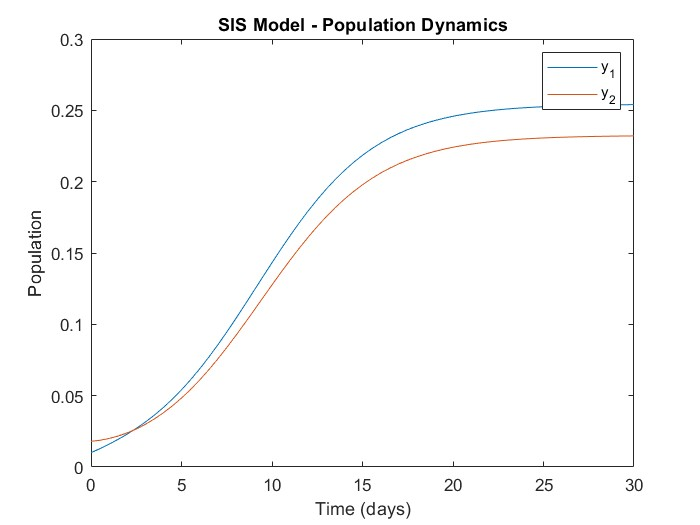
\includegraphics[width=\textwidth]{immagini/PopDynamics1.jpg}
		\label{fig:immagine1}
	\end{minipage}
	\hfill
	% Seconda immagine
	\begin{minipage}{0.45\textwidth}
		\centering
		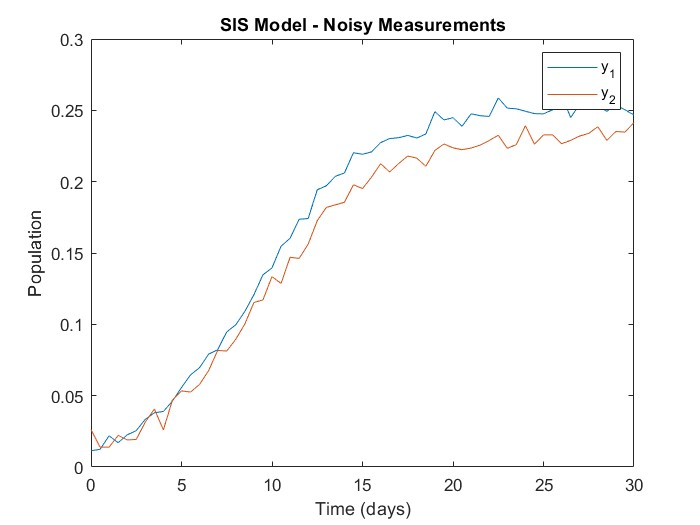
\includegraphics[width=\textwidth]{immagini/PopDynamics2.jpg}
		\label{fig:immagine2}
	\end{minipage}
\end{figure}
\begin{figure}[h]
	\centering
	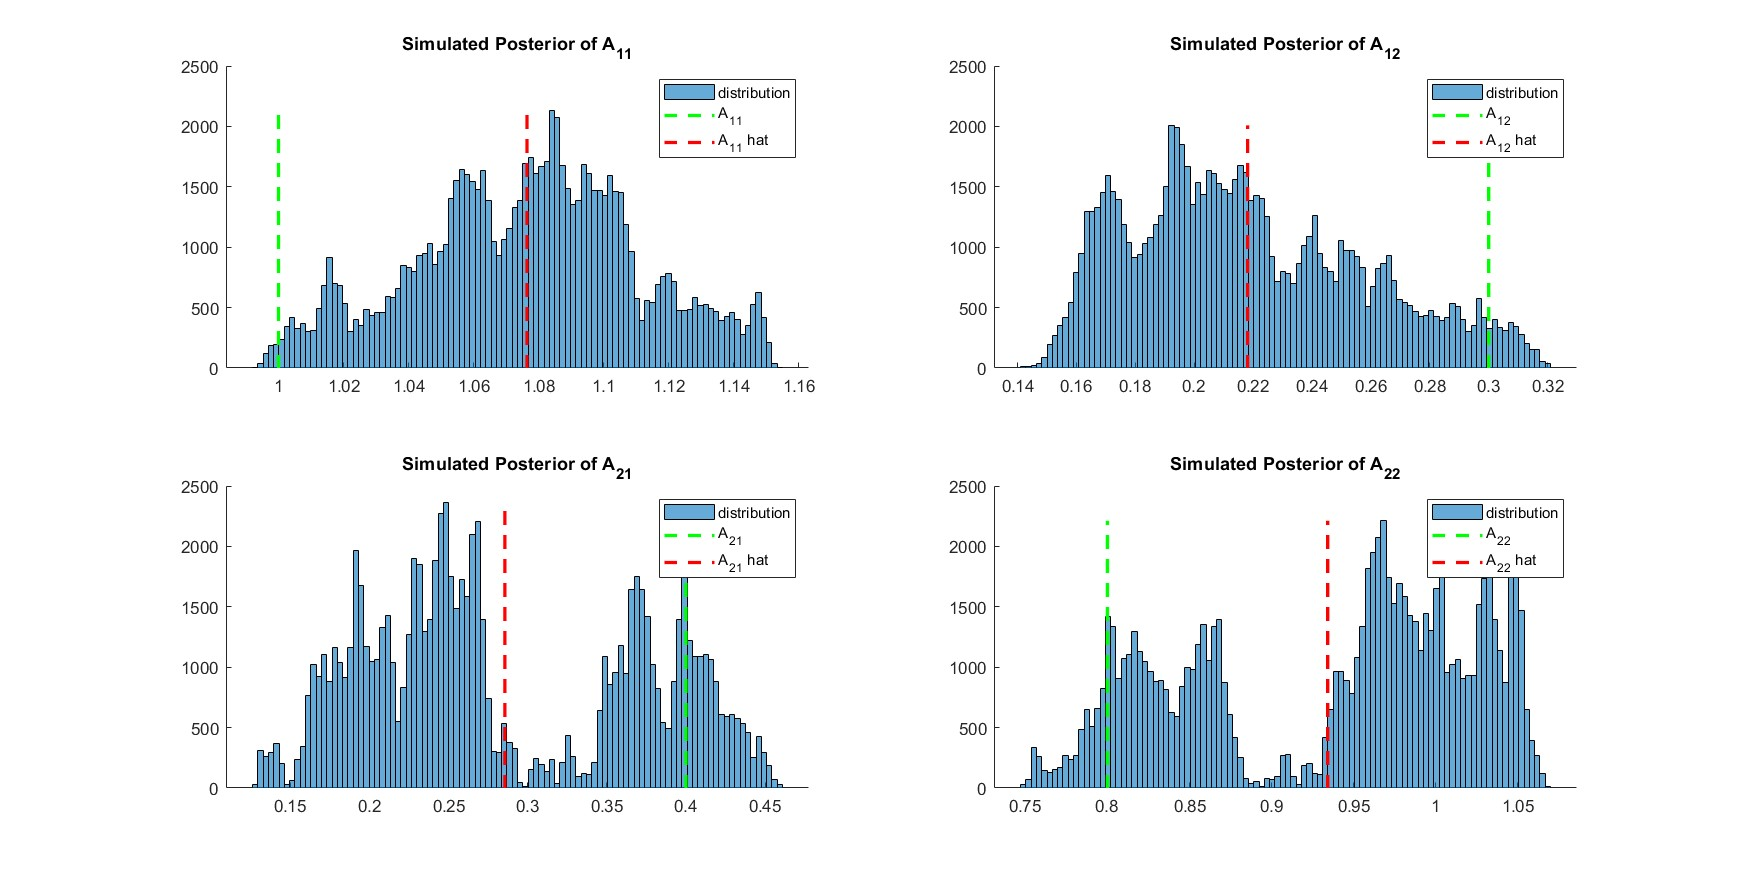
\includegraphics[width=\linewidth]{immagini/Posterior.jpg}
\end{figure}


\section{Discussion}


\section{Conclusion}

This paper explored the dynamics of a deterministic SIS epidemic model over a simple two-node contact network. By numerically simulating the continuous-time nonlinear system, we analyzed the transient and steady-state behaviors of disease propagation starting from small initial infection levels. The results demonstrated how the infection evolves over time depending on the recovery rate and the structure of the contact matrix. Even in a minimal network, we observed complex dynamics, including different steady-state infection levels across nodes, emphasizing the importance of network heterogeneity in epidemic outcomes.

Our findings align with general principles in network epidemic theory, showing how the topology of interactions (i.e., who contacts whom) can significantly influence whether the disease dies out or becomes endemic. While we considered a static network and a basic SIS framework, this work provides a foundation for studying more complex models, including SIR and time-varying networks.

Future work could expand this model to larger networks, incorporate stochastic effects, or investigate optimal intervention strategies. Furthermore, extending this analysis to SIR dynamics or multi-patch models could offer deeper insights into realistic epidemic scenarios where recovery leads to immunity or individuals move between subpopulations.


\section*{References}


Pillonetto, G., Sparacino, G., \& Cobelli, C. (2003).
\textit{Numerical non-identifiability regions of the minimal model of glucose kinetics: superiority of Bayesian estimation}.
Mathematical Biosciences.\\ \\
Gelman, A., Carlin, J. B., Stern, H. S., \& Rubin, D. B. (1995).
\textit{Bayesian Data Analysis}.
Chapman and Hall.\\ \\
Cognome, N. (Anno). *Titolo dell'opera in corsivo*. Casa editrice.

\end{document}
